\documentclass[12pt]{scrartcl}
\usepackage[italian]{babel}
\usepackage[utf8]{inputenc}
\usepackage[T1]{fontenc}
\usepackage[Algoritmo]{algorithm}
\usepackage{algorithmic}
\usepackage{amsmath,amsfonts,amssymb}
\usepackage{mathtools}
\usepackage{tikz}
\usepackage{caption}
\usepackage{float}
\usepackage{enumitem}
\usepackage{pgfplots}
\usepackage{hyperref}
\usepackage{listings}
\usepackage{xcolor}

\usetikzlibrary{arrows, positioning, automata, shapes}
\newcommand{\ceill}[1]{\lceil #1 \rceil}

\title{Verifica delle proprietà dei grafi di Kronecker}
\author{Irene Dini}
\date{\today}

\lstdefinelanguage{mylanguage}{
    keywords={input, output, while, do, end, return, repeat}
    %keywordstyle=\color{red}
 }

\lstdefinestyle{mystyle}{
	language = mylanguage,
	basicstyle=\linespread{1.8}\sffamily\footnotesize,
    keywordstyle=\color{purple}\bfseries,
    stringstyle=\color{red},
    commentstyle=\color{verde},
    morecomment=[s][\color{blue}]{/**}{*/},
    %extendedchars=true,
    showspaces=false,
    showstringspaces=false,
    breaklines=true,
    backgroundcolor=\color{cyan!10},
    breakautoindent=true,
    captionpos=b,
    xleftmargin=0pt,
    tabsize=2
}


\begin{document}
\maketitle
\newpage

\section{Introduzione}

Questo progetto illustra alcuni esperimenti effettuati su grafi di Kronecker: lo scopo è quello di verificare se essi rispettano alcune proprietà che caratterizzano la rete sociale a partire dalla quale sono stati generati. Ci siamo concentrati in particolare sulla distribuzione dei gradi e sul coefficiente di clustering. Dato che quest'ultima quantità è definita solo per nodi di grafi non diretti, abbiamo preso in considerazione due reti sociali non dirette.

\subsection{Strumenti utilizzati}

Gli strumenti utilizzati per questo progetto sono python per il pre-processing, l'elaborazione e la visualizzazione dei dati, e gli algoritmi \textsf{KRONFIT} e \textsf{KRONGEN} disponibili su \href{http://snap.stanford.edu/snap/download.html}{Snap Stanford}.

\subsubsection{KRONFIT}
\textsf{KRONFIT} è l'algoritmo che, presa in input la lista di archi del grafo $\mathcal{G}$ da ``simulare'' e la dimensione desiderata $N_1$, stima l'\textit{initiator matrix} $\mathbf{K_1}$ (di dimensione $N_1\times N_1$) da cui generare il grafo di Kronecker, utilizzando il metodo della discesa del gradiente e l'algoritmo di Metropolis. Lo pseudocodice è riportato nel seguente listato:

\begin{lstlisting}[mathescape=true, style=mystyle]
input: size of parameter matrix $N_1$, graph G, and learning rate $\lambda$
output: MLE parameters $\hat{\Theta}(N_1\times N_1$ probability matrix)

initialize $\hat{\Theta}$
while not converged do
	evaluate gradient: $\frac{\delta}{\delta\hat{\Theta}_t}l(\hat{\Theta}_t)$
	update parameter estimates: $\hat{\Theta}_{t+1} = \hat{\Theta}_t+\lambda\frac{\delta}{\delta\hat{\Theta}_t}l(\hat{\Theta}_t)$
end
return $\hat{\Theta} = \hat{\Theta}_t$
\end{lstlisting}

Per come è strutturato l'algoritmo, se si lavora con grafi non diretti è necessario un leggero pre-processing: sia
\[EL = \{(v_0, v_1), (v_2, v_3), \ldots, (v_{n-1}, v_{n})\}\]
la lista degli archi del grafo $G$, per ogni arco $(v_i, v_j)\in EL$, bisogna inserire in $EL$ anche $(v_j, v_i)$.

\subsubsection{KRONGEN}
\textsf{KRONGEN} è invece l'algoritmo che, data l'\textit{initiator matrix} $\mathbf{\hat{\Theta}}$ di dimensione $N_1\times N_1$ ed il numero di iterazioni da eseguire $k$, genera un grafo con $N_1^k$ nodi, la cui matrice di adiacenza è appunto la matrice di Kronecker $\mathbf{K_k} =\underbrace{\mathbf{K_1}\otimes \mathbf{K_1}\otimes \ldots \otimes \mathbf{K_1}}_\text{k volte}$. Il numero di iterazioni viene calcolato secondo la regola: $N_1^{k-1}<N(G)\leq N^k_1$. Indichiamo con $\mathbf{\hat{\Theta}} = \{\theta_{ij}\}$ e $E_1 = \sum_{ij}\theta_{ij}$

\begin{lstlisting}[mathescape=true, style=mystyle]
input: Initiator matrix $\hat{\Theta}$, number of iterations $k$
output: Kronecker Matrix $\mathbf{K_k}$ with $N_1^k$ nodes

repeat $E_1^k$ times
	sample edge: simulate the Kronecker product $k$ times, each time choosing an edge from $\hat{\Theta}$ with probability $\frac{\theta_{ij}}{E_1}$
	add edge to $\mathbf{K_k}$
return $\mathbf{K_k}$
\end{lstlisting}

La matrice restituita avrà un numero di nodi che tende a $E_1^k$. In questo caso è però necessario del post-processing: anche se la matrice $\mathbf{\hat{\Theta}}$ è simmetrica, data la natura probabilistica del processo, è molto poco probabile che il grafo di Kronecker ottenuto risulterà essere non diretto. Per renderlo tale, basta semplicemente considerare solo gli archi $(v_i, v_j)$ con $i\leq j$. Questa operazione equivale a considerare solo la parte triangolare inferiore della matrice di adiacenza del grafo.\\
\textbf{NB}: In realtà si potrebbe anche cosiderare la parte triangolare superiore: da un'unica matrice di Kronecker ``diretta'', si possono generare due grafi non diretti.

\section{Esperimenti}
Le reti sociali su cui abbiamo scelto di lavorare sono non dirette e non pesate.

\subsection{Grafo di Facebook}

La prima rete sociale presa in considerazione è una parte del grafo di Facebook disponibile su \href{http://snap.stanford.edu/data/egonets-Facebook.html}{Snap Stanford}. Le sue caratteristiche sono le seguenti:
\begin{itemize}
	\item Nodi: 4039
	\item Archi: 88234
	\item Diametro: 8
	\item Nodi GCC: 4039
	\item Grado medio: 43.6910
\end{itemize}
 Dopo il pre-processing abbiamo applicato \textsf{KRONFIT} e \textsf{KRONGEN} per ottenere $4$ diversi grafi di Kronecker e confrontare le loro caratteristiche con quelle del grafo di partenza. 


\subsubsection{Kronfit}
Per prima cosa abbiamo applicato \textsf{KRONFIT} al grafo di Facebook, per ottenere una initiator matrix di dimensione $2\times2$ e una di dimensione $3\times3$:

\[ \mathbf{\hat{\Theta}_2} = \begin{pmatrix}
0.9999 & 0.691526 \\
0.691459 & 0.349524 
\end{pmatrix}  \]

\[ \mathbf{\hat{\Theta}_3} = \begin{pmatrix}
0.4372 & 0.6576 & 0.08469 \\
0.6544 & 0.9999 & 0.3151 \\
0.084 & 0.3151 & 0.9999 
\end{pmatrix}  \]

Come ci si poteva aspettare, dato che il grafo in ingresso è non diretto, entrambe le matrici risultano praticamente simmetriche.

\subsubsection{Krongen}
A partire dalle \textit{initiator matrix}, dopo aver calcolato il numero di iterazioni da fare, abbiamo applicato \textsf{KRONGEN} per ottenere dei grafi di Kronecker.  Studiamo i due casi separatamente. \\
Per quanto riguarda $\mathbf{\hat{\Theta}_2}$ si ha che:
\begin{center}
	$k = 12$ infatti: $2^{11} = 2048 < 4039 \leq 4096 = 2^{12}$
\end{center}
Il grafo $\mathcal{G}_2$ ottenuto, dopo il post-processing, ha le seguenti caratteristiche:
\begin{itemize}
	\item Nodi: $4096$ 
	\item Archi: $86365$ ($173200$ prima del post-porocessing)
	\item Diametro: $5$
	\item Nodi GCC: $4096$
	\item Grado medio: $42.1704$
\end{itemize}
Escludendo il diametro, che risulta essere piuttosto più piccolo, tutte le quantità stimate si avvicinano molto a quelle del grafo di partenza.\\
Per quanto riguarda $\mathbf{\hat{\Theta}_3}$ invece:
\begin{center}
	$k = 8$ infatti: $3^7 = 2187< 4039 \leq 6561 = 3^8$
\end{center}
Le caratteristiche del grafo $G_3$ sono:
\begin{itemize}
	\item Nodi: $6561$ 
	\item Archi: $91346$ ($183012$ prima del post-porocessing)
	\item Diametro: $5$
	\item Nodi GCC: $6561$
	\item Grado medio: $27.8451$
\end{itemize}
In questo caso notiamo subito che le caratteristiche del grafo di Kronecker sono abbastanza lontane da quelle del grafo di partenza: il numero di nodi ed il numero di archi risultano essere più alti, mentre il diametro ed il grado medio sono molto più bassi.
\subsection{Studio delle proprietà}
Abbiamo fatto uno studio grafico della distribuzione dei gradi e del coefficiente di clustering, per vedere quanto i grafi $\mathcal{G}_2$ e $\mathcal{G}_3$ si avvicinassero al grafo originario $\mathcal{G}$. Il grafico \ref{fig:fig1} rappresenta la distribuzione dei gradi dei 3 grafi: ad ogni grado è associato il numero di nodi che hanno quel grado.

\begin{figure}[H]
	\centering
	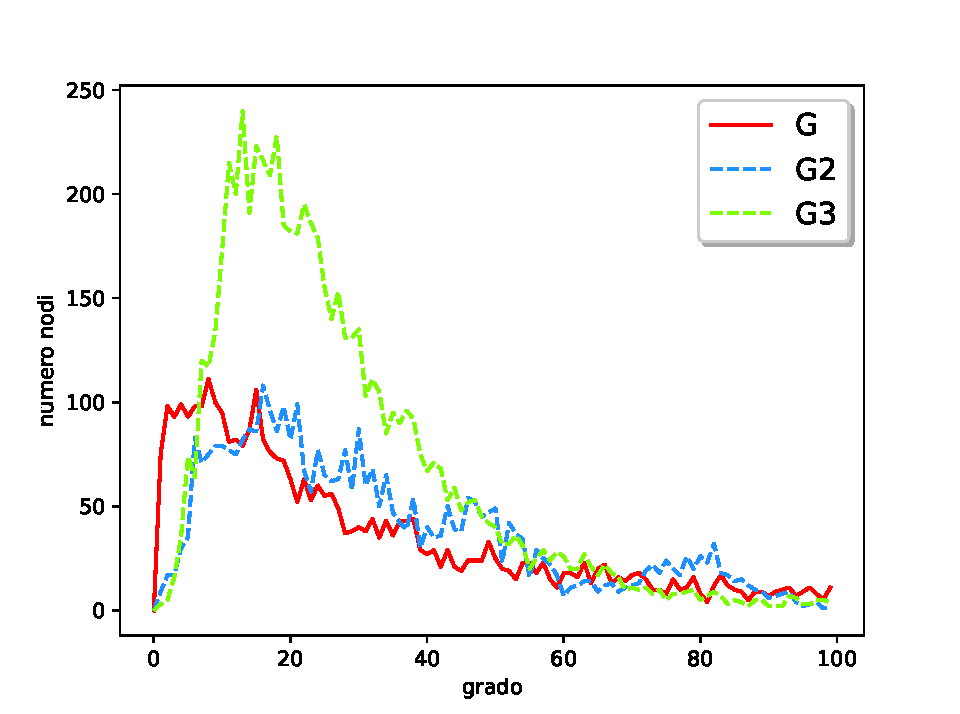
\includegraphics[width=0.7\linewidth]{imgs/Figure_1.pdf}
	\caption{Distribuzione dei gradi}\label{fig:fig1}
\end{figure}

Come si può notare, la distribuzione dei gradi di $\mathcal{G}_2$ non si discosta molto da quella di $\mathcal{G}$, si ha una differenza sostanziale solo per i gradi che vanno da $1$ a $5$. La distribuzione dei gradi di $\mathcal{G}_3$ è invece molto diversa.\\
Vediamo adesso se queste distribuzioni seguono una power-law, trasferendo il grafico in scala logaritmica (Figura \ref{fig:fig2}). 
\begin{figure}[H]
	\centering
	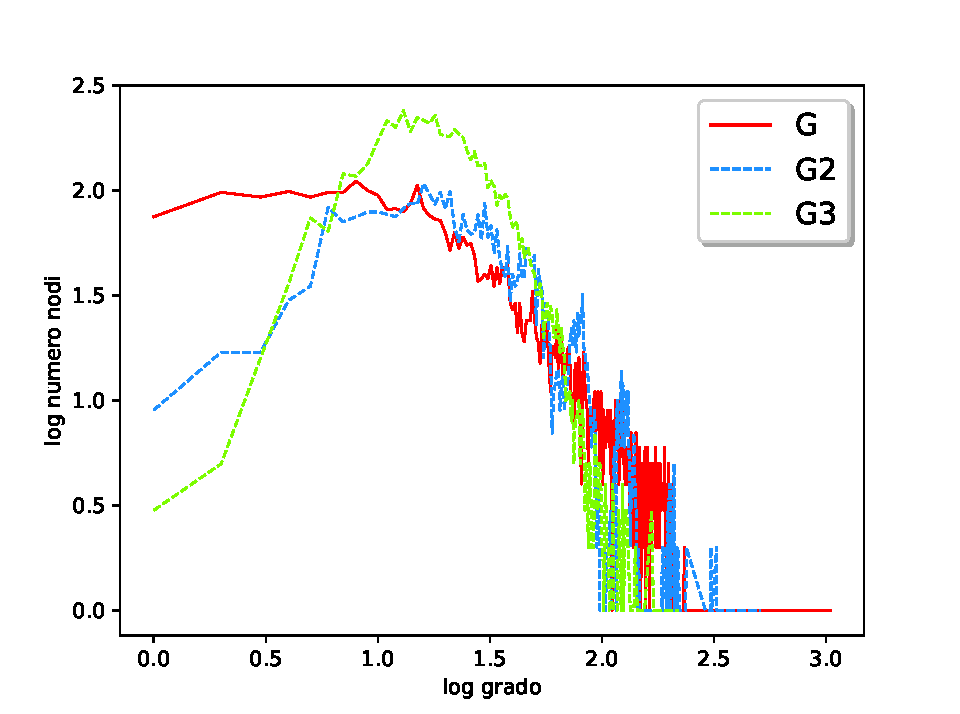
\includegraphics[width=0.7\linewidth]{imgs/Figure_2.pdf}
	\caption{Degree Power-Law}\label{fig:fig2}
\end{figure}

L'andamento dei $3$ grafici è molto simile: da $1.3$ circa in poi, anche se molto oscillatorio, ricorda una retta. Non si può comunque concludere che i grafi di Kronecker seguano una power law ma, dato che non la seguiva nemmeno il grafo di partenza, era prevedibile.\\

Come ultima cosa, abbiamo confrontato i coefficienti di clustering dei nodi. Nel grafico in figura \ref{fig:fig3} ad ogni nodo è associato il suo coefficiente di clustering (in ordine decrescente per questo valore).

\begin{figure}[H]
	\centering
	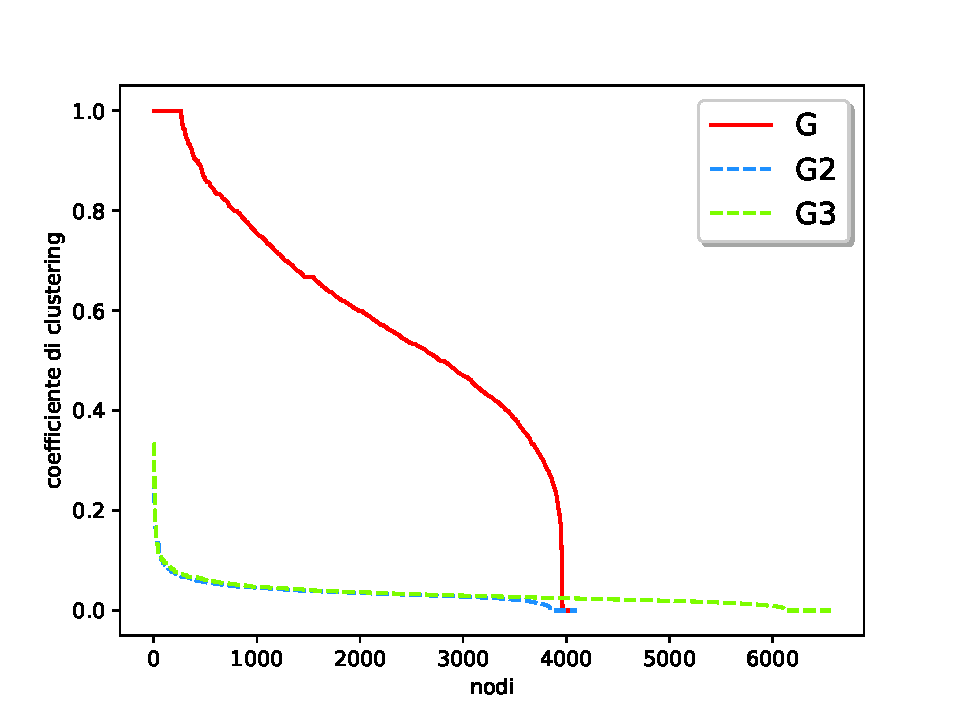
\includegraphics[width=0.7\linewidth]{imgs/Figure_3.pdf}
	\caption{Clustering coefficient}\label{fig:fig3}
\end{figure}

Mentre negli altri due casi $\mathcal{G}_2$ approssimava almeno qualitativamente la distribuzione dei gradi del grafo $\mathcal{G}$, in questo caso si ottiene una distribuzione totalmente differente.\\~\\
Riportiamo di seguito altri esempi, per vedere se, partendo da sampling diversi, si potessero ottenere risultati migliori. Nei grafici riportati nelle figure \ref{fig:fig4} e \ref{fig:fig5} si confronta quindi il grafo $\mathcal{G}_2$ (che portava una migliore approssimazione di $\mathcal{G}$ rispetto a $\mathcal{G}_3$), con altri due grafi generati sempre a partire da una \textit{initiator matrix} di dimensione $2\times2$. $\mathcal{G}_{2.1}$ è semplicemente un altro sampling di $\mathbf{\hat{\Theta}_2}$ e le sue caratteristiche sono:
\begin{itemize}
	\item Nodi: $4093$ 
	\item Archi: $91346$ ($173200$ prima del post-porocessing)
	\item Diametro: $5$
	\item Nodi GCC: $4093$
	\item Grado medio: $42.5121$
\end{itemize}
 
Per $\mathcal{G}_{2.2}$ è stato invcee nuovamente eseguito \textsf{KRONFIT} ottenendo la matrice
\[
	\mathbf{\hat{\Theta}_{2.2}} =
	\begin{pmatrix}
	0.9999 & 0.6914 \\
	0.6914 & 0.3501 
	\end{pmatrix} 
\]
Da essa, applicando \textsf{KRONGEN} si è ottenuto un grafo con le seguenti caratteristiche:

\begin{itemize}
	\item Nodi: $4093$ 
	\item Archi: $86763$ ($173421$ prima del post-porocessing)
	\item Diametro: $5$
	\item Nodi GCC: $4093$
	\item Grado medio: $42.3958$
\end{itemize}

In entrambi i casi, le caratteristiche elencate sono molto vicine a quelle di $\mathcal{G}_2$ e quindi di $\mathcal{G}$.\\
Le figure \ref{fig:fig4} e \ref{fig:fig5} mostrano come l'andamento dei gradi e del coefficiente di clustering di questi due grafi siano molto simili a quelli di $\mathcal{G}_2$. Questo porta a pensare che non potremo ottenere approssimazioni di $\mathcal{G}$ molto migliori utilizzando i grafi di Kronecker.

\begin{figure}[H]
	\centering
	\begin{minipage}{.5\textwidth}
		  \centering
		  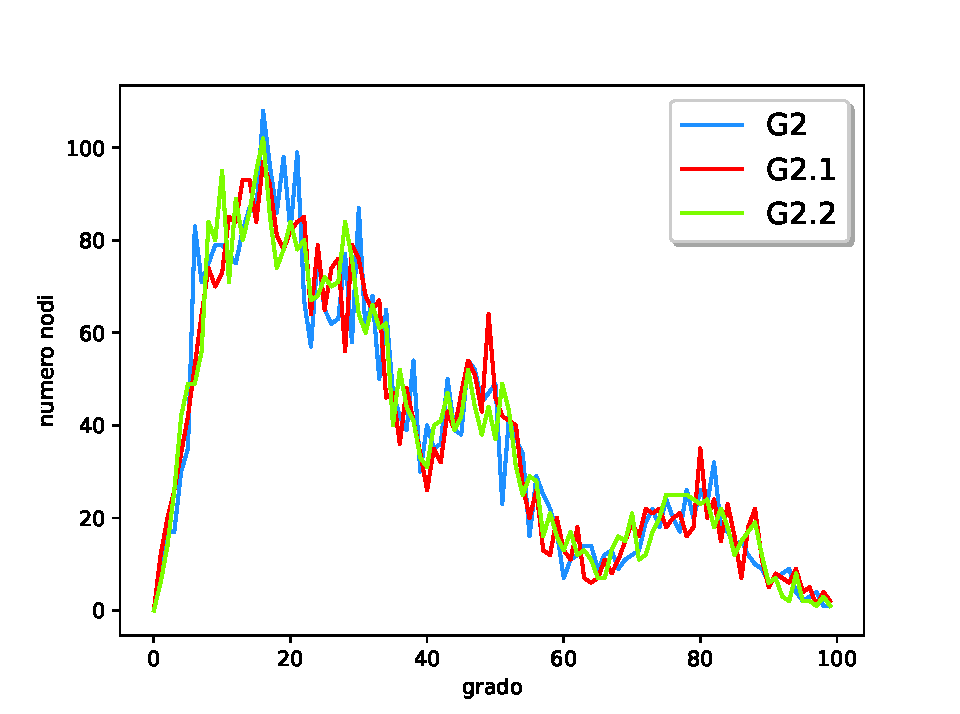
\includegraphics[width=1\linewidth]{imgs/Figure_4.pdf}
		  \caption{Distribuzione dei gradi}\label{fig:fig4}
	\end{minipage}%
	\begin{minipage}{.5\textwidth}
		  \centering
		  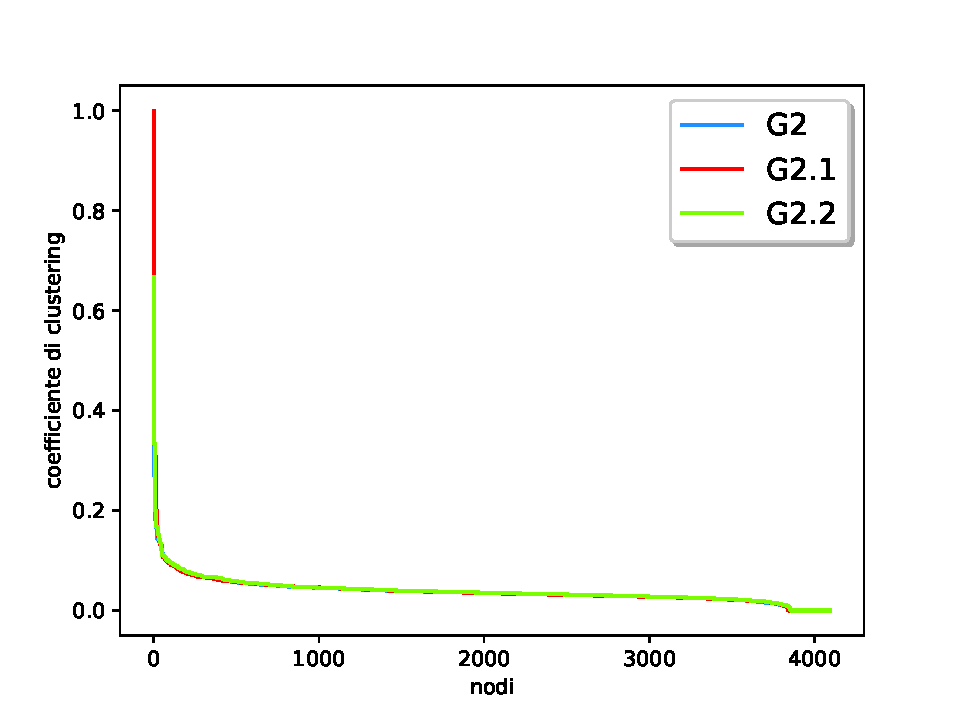
\includegraphics[width=1\linewidth]{imgs/Figure_5.pdf}
		  \caption{Coefficiente di clustering}\label{fig:fig5}
	\end{minipage}
\end{figure}


\subsection{Grafo citazioni}

La seconda rete considerata è Arxiv GR-QC (General Relativity and Quantum Cosmology), una rete di citazioni disponibile su \href{http://snap.stanford.edu/data/ca-GrQc.html}{Snap Stanford}. Rappresenta le collaborazioni tra gli autori che hanno scritto articoli per GR-QC: se un autore $i$, ha scritto un articolo insieme all'autore $j$, il grafo contiene un arco non diretto tra $i$ e $j$. Le caratteristiche di questa rete sono:
\begin{itemize}
	\item Nodi: $5242$
	\item Archi: $14496$
	\item Diametro: $17$
	\item Nodi GCC: $4158$
	\item Grado medio: $5.5307$
\end{itemize}

\subsubsection{Kronfit}

Dopo il pre-processing, abbiamo applicato l'algoritmo di \textsf{KRONFIT} per ottenere una \textit{initiator matrix} di dimensione $2\times2$ e una di dimensione $3\times3$, cioè:
\[
	\mathbf{\hat{\Theta}_2} = 
	\begin{pmatrix}
		0.9999 & 0.3624 \\
		0.3624 & 0.4497 
	\end{pmatrix}
\]

\[
	\mathbf{\hat{\Theta}_3} =
	\begin{pmatrix}
		0.3631 & 0.5434 & 0.01157 \\
		0.5434 & 0.6927 & 0.1968 \\
		0.01157 & 0.197 & 0.9999 
	\end{pmatrix}  
\]

Come ci si doveva aspettare, anche in questo caso le matrici ottenute sono simmetriche, in quanto il grafo di partenza è non diretto.

\subsubsection{Krongen}
Per prima cosa è necessario calcolare il numero di iterazioni $k$, basandosi sul numero di nodi del grafo di partenza. Per quanto riguarda $\mathbf{\hat{\Theta}_2}$ si ha che:

\begin{center}
	$k = 13$ infatti: $2^{12} = 4096 < 5242 \leq 8192 = 2^{13}$
\end{center}

Applicando \textsf{KRONGEN} abbiamo ottenuto il grafo $G_2$ con le seguenti caratteristiche:
\begin{itemize}
	\item Nodi: $6451$ ($8192$ prima del post-processing)
	\item Archi: $12181$ ($24289$ prima del post-porocessing)
	\item Diametro: $16$
	\item Nodi GCC: $6119$
	\item Grado medio: $3.7765$
\end{itemize}

Il numero di nodi risulta essere piuttosto maggiore di quello di $\mathcal{G}$ (dovevamo aspettarcelo dato che non esiste una potenza di $2$ vicina a $5242$), e notiamo come sarebbe stato ancora maggiore se avessimo avuto a che fare con un grafo diretto. Il grado medio ed il numero di archi risultano invece più piccoli.\\
Per $\mathbf{\hat{\Theta}_3}$ si ha invece che:

\begin{center}
	$k = 8$ infatti: $3^{12} = 2187 < 5242 \leq 6561 = 3^{8}$
\end{center}

Applicando \textsf{KRONGEN} abbiamo ottenuto il grafo $\mathcal{G}_3$ con le seguenti caratteristiche:

\begin{itemize}
	\item Nodi: $6158$ ($6561$ prima del post-processing)
	\item Archi: $12738$ ($24766$ prima del post-porocessing)
	\item Diametro: $15$
	\item Nodi GCC: $6130$
	\item Grado medio: $4.1371$
\end{itemize}
Le caratteristiche di questo grafo sono simili a quelle del precedente.\\

Il grafo $\mathcal{G}_2$ prima del post-processing aveva un numero di nodi molto maggiore rispetto a $\mathbf{G}$, ma rendendolo non diretto, dato che non vengono considerati i nodi di grado $0$, produce un'approssimazione più precisa.

\subsection{Studio delle proprietà}
Come per il grafo di Facebook abbiamo per prima cosa studiato l'andamento dei gradi, mettendo a confronto quelle di $\mathcal{G}$, $\mathcal{G}_2$ e $\mathcal{G}_3$, in figura \ref{fig:fig6}
\begin{figure}[H]
	\centering
	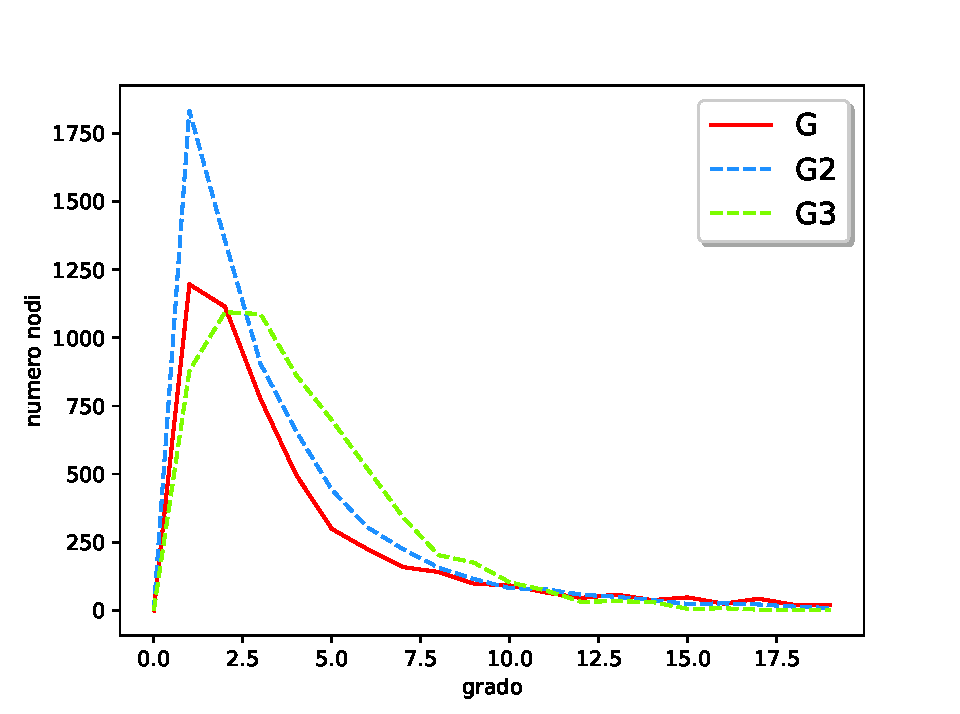
\includegraphics[width=0.7\linewidth]{imgs/Figure_6.pdf}
	\caption{Distribuzione dei gradi}\label{fig:fig6}
\end{figure}

Sono riportati solo i primi $20$, in quanto l'andamento dei successivi è praticamente identico per le $3$ reti. Notiamo come $\mathcal{G}_2$ abbia un numero di nodi di grado $1$ molto più alto di $\mathcal{G}$ ma, per il resto, la sua distribuzione risulti essere una buona approssimazione. La distribuzione di $\mathcal{G}_3$ risulta invece essere abbastanza spostata verso destra, mostrando che il grafo ha, in generale, molti più nodi di grado compreso tra $3$ e $5$ rispetto a $\mathcal{G}$.\\
Verifichiamo adesso se queste distribuzioni seguono una power-law: in figura \ref{fig:fig7} è riportato il grafico precedente in scala logaritmica.

\begin{figure}[H]
	\centering
	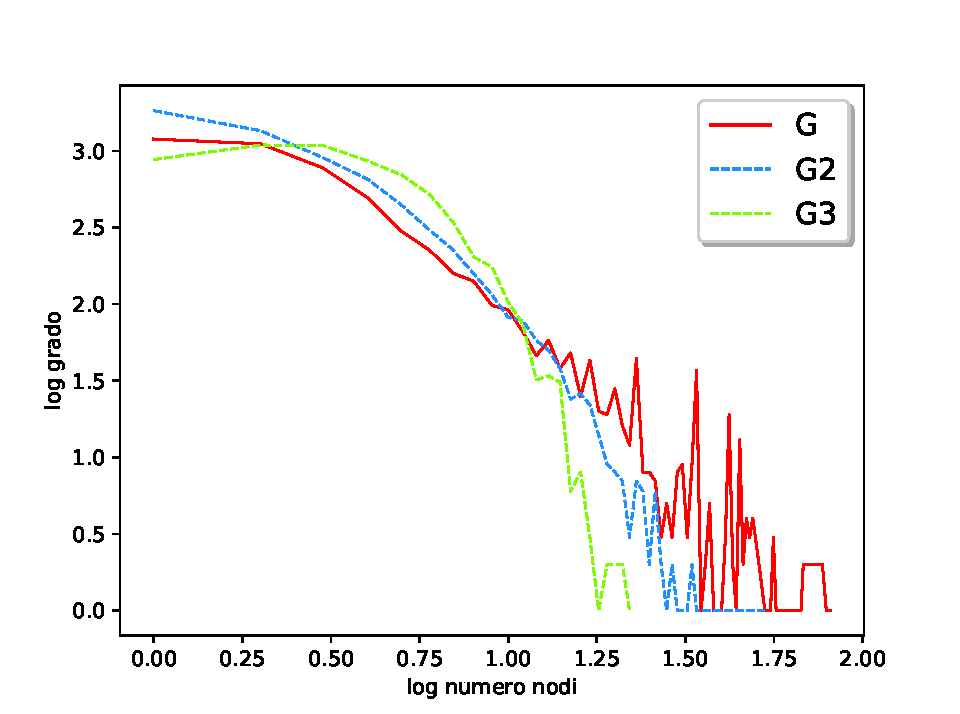
\includegraphics[width=0.7\linewidth]{imgs/Figure_7.pdf}
	\caption{Power-law}\label{fig:fig7}
\end{figure}

La figura mostra come i grafi di Kronecker seguano una degree power-law in modo più fedele rispetto al grafo originale.\\
Come ultima cosa verifichiamo la distribuzione dei coefficienti di clustering. La figura \ref{fig:fig8}, come per il grafo di Facebook, associa ad ogni nodo il suo coeffciente di clustering, ordinandoli in modo decrescente. Anche questa volta risulta essere totalmente diversa da quella del grafo di partenza.

\begin{figure}[H]
	\centering
	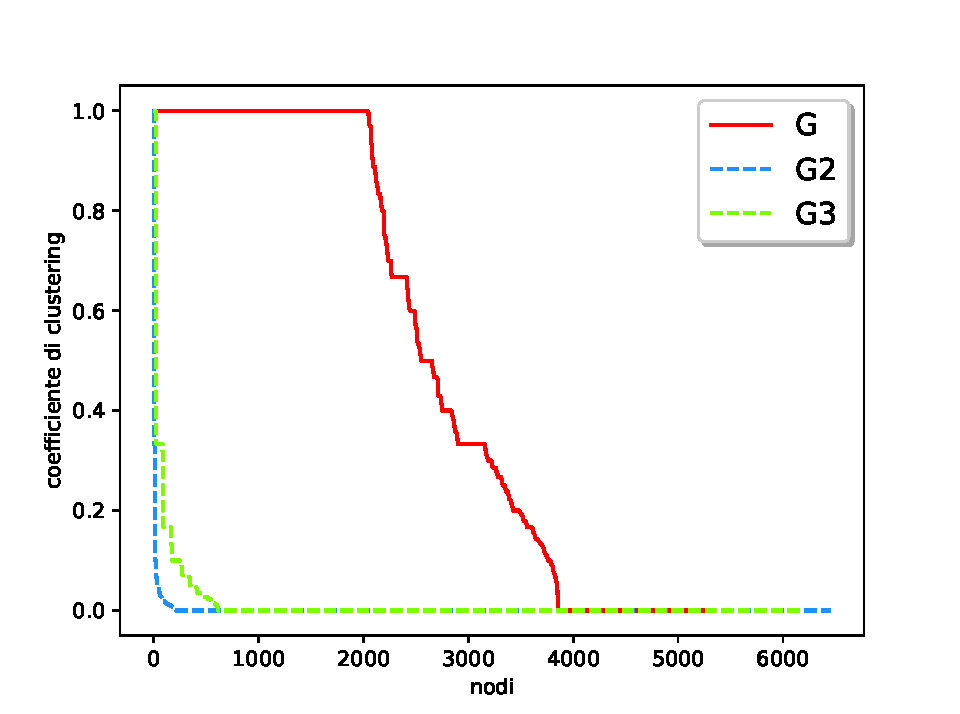
\includegraphics[width=0.7\linewidth]{imgs/Figure_8.pdf}
	\caption{Coefficiente di clustering}\label{fig:fig8}
\end{figure}


\section{Conclusioni}

Dagli esperimenti condotti si può dedurre che, in realtà, almeno per reti di dimensioni piuttosto contenute, i grafi di Kronecker non producono approssimazioni soddifacenti. Anche semplicemente confrontando caratteristiche ``semplici'' come il grado medio e il diametro, non è detto che si ottengano valori uguali a quelli del grafo originale. Inoltre, mentre per la distribuzione dei gradi, i grafi di Kronecker ricordano almeno qualitativamente l'andamento del grafo di origine, per quanto riguarda il coefficiente di clustering, si ottengono distribuzioni totalmente diverse dalla sua, indipendentemente dai parametri utilizzati per stimare il modello di generazione.

\end{document}

  